%!TEX root = paper.tex
\section{Results from Initial Evaluations}
\label{sec:evaluation}

% Furthermore, as these benchmarks are in the process of being evaluated on different platforms, the results presented here may not appear to be uniform across benchmarks.

In this section, we present some of the early results obtained initial evaluations of our benchmarks. As this is the first time we are presenting these findings, it is worth noting that the initial evaluations are far from being complete or perfect, especially when lacking any relative measures to benchmark against. However, these initial evaluations are likely to provide more insight into how these evaluations should be tuned or scoped in future releases.  We outline these aspects in Table~\ref{tab:eval-summary}. We relied on three different platforms, namely,  Pearl\footnote{\url{https://www.turing.ac.uk/research/asg/pearl}}, Summit\footnote{\url{https://www.olcf.ornl.gov/summit/}} and Theta\footnote{\url{https://www.alcf.anl.gov/alcf-resources/theta}}, along with other architectures, for our evaluations.

\begin{small}
\begin{table}
    \caption{Summary of the Evaluation.}
    \label{tab:eval-summary}
    \centering
    \begin{tabular}{|l|l|l|l|}
        \hline
        {\bf Benchmark}	& {\bf Platforms}		 & {\bf Science }   & {\bf Performance}\\
                    	& {\bf /(Architectures)} & {\bf Metric(s)}  & {\bf Metric(s)}\\
        \hline
        \hline
        {\tt cloud-mask}	& Pearl (V100) 		& Accuracy			& Scalability\\
                        	& Summit (V100)		&       			& \\
        \hline
        {\tt stemdl}		& Summit (V100)		& Accuracy, F1		& -\\
        \hline
        {\tt candle-uno}	& Theta (A100)		& -					& Throughput\\
        \hline
        {\tt tevelop}		& K80, P100, V100        & NNSE		        & Training Time\\
                    		& A100, RTX3080, RTX3090	&                   & \\
        \hline
        \hline
    \end{tabular}
 \end{table}
\end{small}

 
%%% Cloud Masking 
\subsection{Results for the {\tt cloud-mask} Benchmark}

We show the masking accuracy for the training and validation cases in Figure~\ref{fig:cm-scalable-1}, and the scalability results in Figure~\ref{fig:pearl-summit}.  We show two different performance results. In the former, we show how the accuracy of the classification varies against the number of epochs, either trained or tested. The latter shows how the benchmark training scales (average time per epoch) on the Pearl and Summit platforms when the number of GPUs are varied up to 32. There are a number of observations here:

\begin{itemize}
    \item The accuracy improves with the number of epochs (both testing and training), but they do not exceed 95\% of the accuracy shows by the Bayesian mask-based ground truth. However, this has to be interpreted very carefully. The Bayesian-based mask is not necessarily the best either~\cite{merchant:2005}. Hence the sub-optimal outputs does not mean, the ML model is not being effective. We are exploring different means for verifying the real accuracy of the model (such as using data from LIDAR and ground sensors). 
    \item Pearl offers better scalability when more than two GPUs are used, while for Summit this has to be four GPUs. However, interestingly, both Pearl and Summit are based on V100 GPUs with totally two different configurations. However, there are performance differences between these platforms when a few GPUs are used. A more detailed investigation is needed both on the scalability and why few GPUs offer sub-optimal performance.  
\end{itemize}

\noindent It is very important to note that these conclusions would not have been possible without these initial evaluations. 


\begin{figure}[!htb]
\begin{subfigure}{0.43\textwidth}
\centering
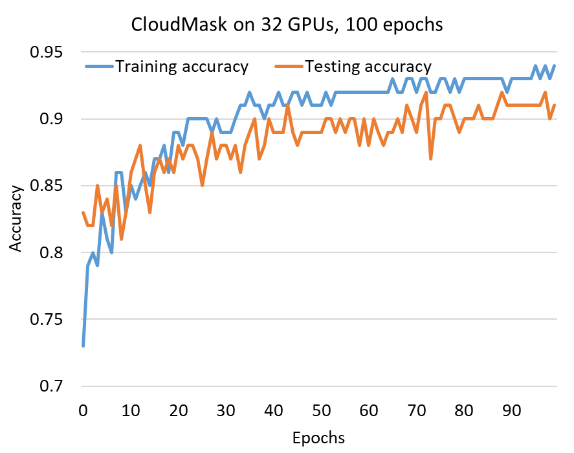
\includegraphics[width=0.9\textwidth]{images/cloudmask/image2.png}
\caption{}
\label{fig:cm-scalable-1}
\end{subfigure}
\hfill
\begin{subfigure}{0.57\textwidth}
\centering
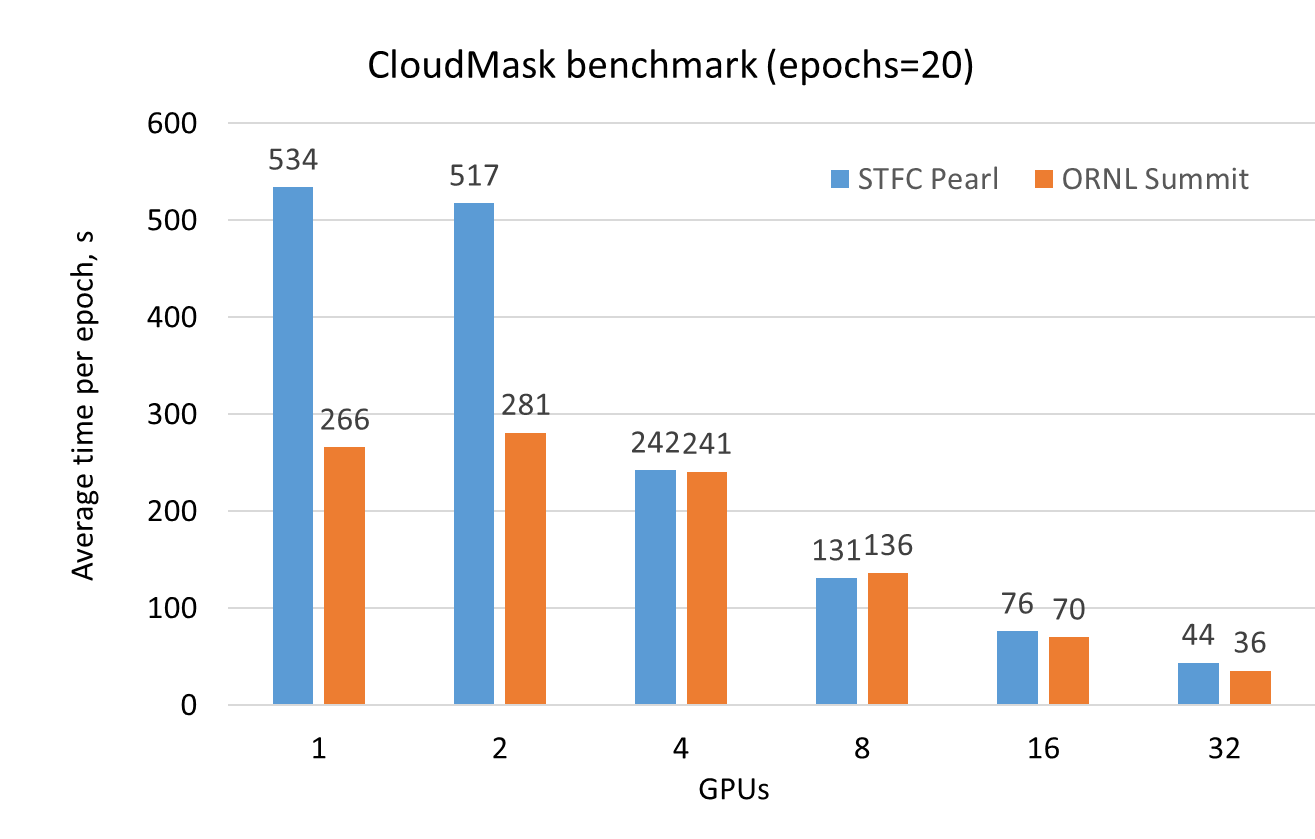
\includegraphics[width=0.9\columnwidth]{images/cloudmask/image3.png}
\caption{}
\label{fig:pearl-summit}
\end{subfigure}
\caption{Performance of {\tt cloud-mask}. The classification accuracy against the number of epochs (on Pearl), and  the training scalability of benchmark both on Pearl and Summit platforms are shown in (a) and (b), respectively.}
\end{figure}





%%% STEMDL

\subsection{Results for the {\tt stemdl} Benchmark}

We used the Namsa simulation code\footnote{\url{https://www.osti.gov/biblio/1631694}} on the Summit to generate CBED patterns for well over  60,000 solid-state materials, representing nearly every known crystal structure, on which we used the reference implementation. Although the classification accuracy is the ultimate metric, this is influenced by a number of hyper-parameters that underpin our network architecture. As such, it is important to ensure that the the best classification is achieved through hyper-parameter search. Although various techniques exist for hyper-parameter search, and that itself can be a separate benchmarking challenge, here we show the validation accuracy and F1-score for various hyper-parameter sets. There are a number of observations here, but to highlight two: first, as expected, hyper-parameters have an overall influence on the rate and best performance of the benchmark, and secondly the performance converges rapidly for some of the hyper-parameter settings, namely, for the ResNet-101 model. We also show how the accuracy can further be improved from baseline performance in Figure~\ref{fig:stemdl6}, where the raw performance is marked as (1), along with various optimizations, including,   pre-processing (2),  time augmentation (3), regularization~(4), and by using deeper models~(5). These optimizations improve the accuracy from 14\% to 57\% through these optimizations. 





\begin{figure}[!htb]
    \begin{subfigure}{0.49\textwidth}
    \centering
    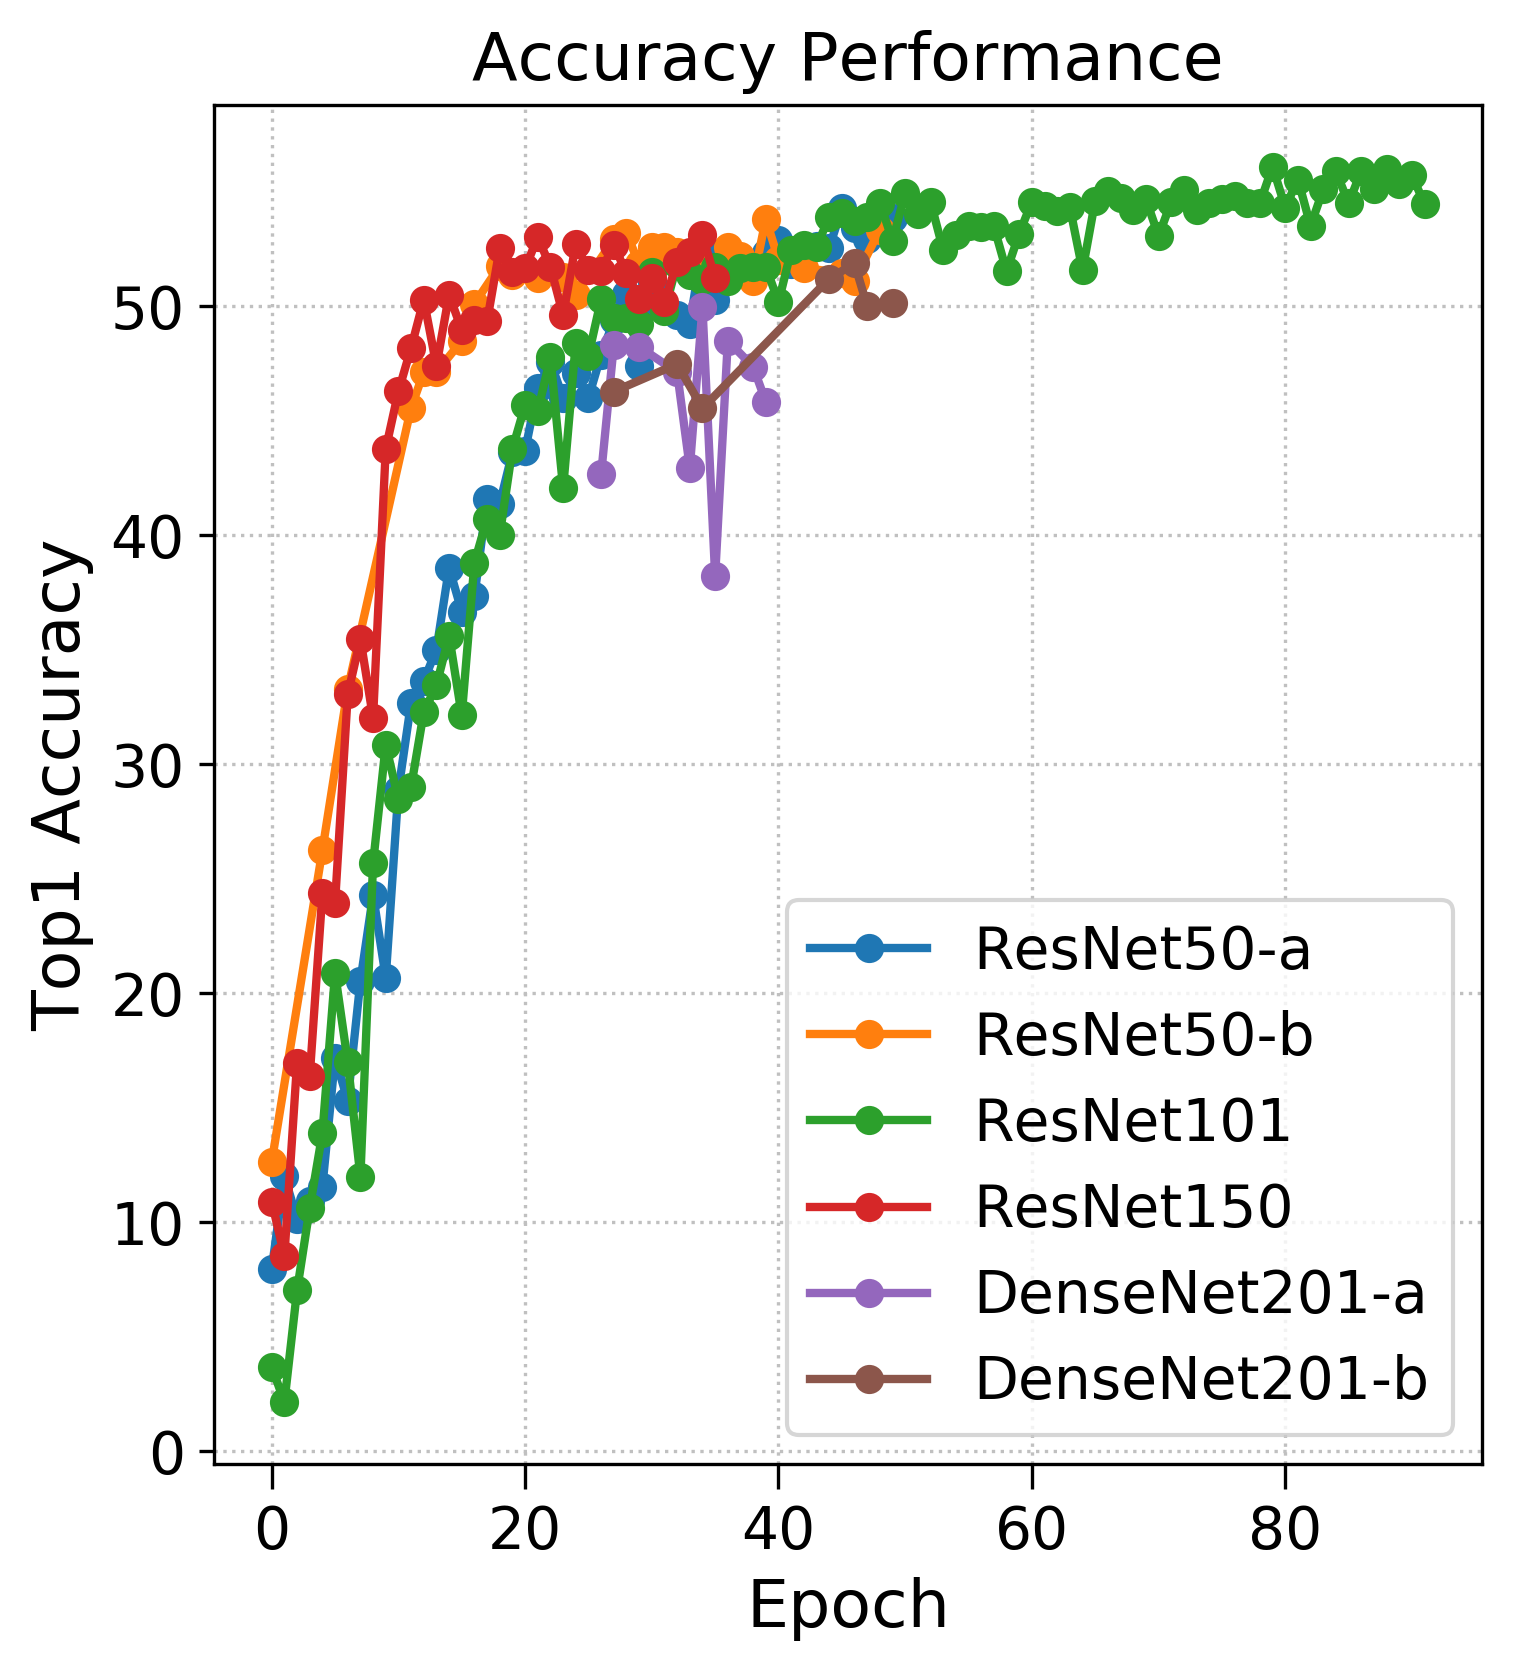
\includegraphics[width=0.9\textwidth]{images/stemdl/image5a.png}
    \caption{}
    \label{fig:stemdl-accuracy}
    \end{subfigure}
    \hfill
    \begin{subfigure}{0.49\textwidth}
    \centering
    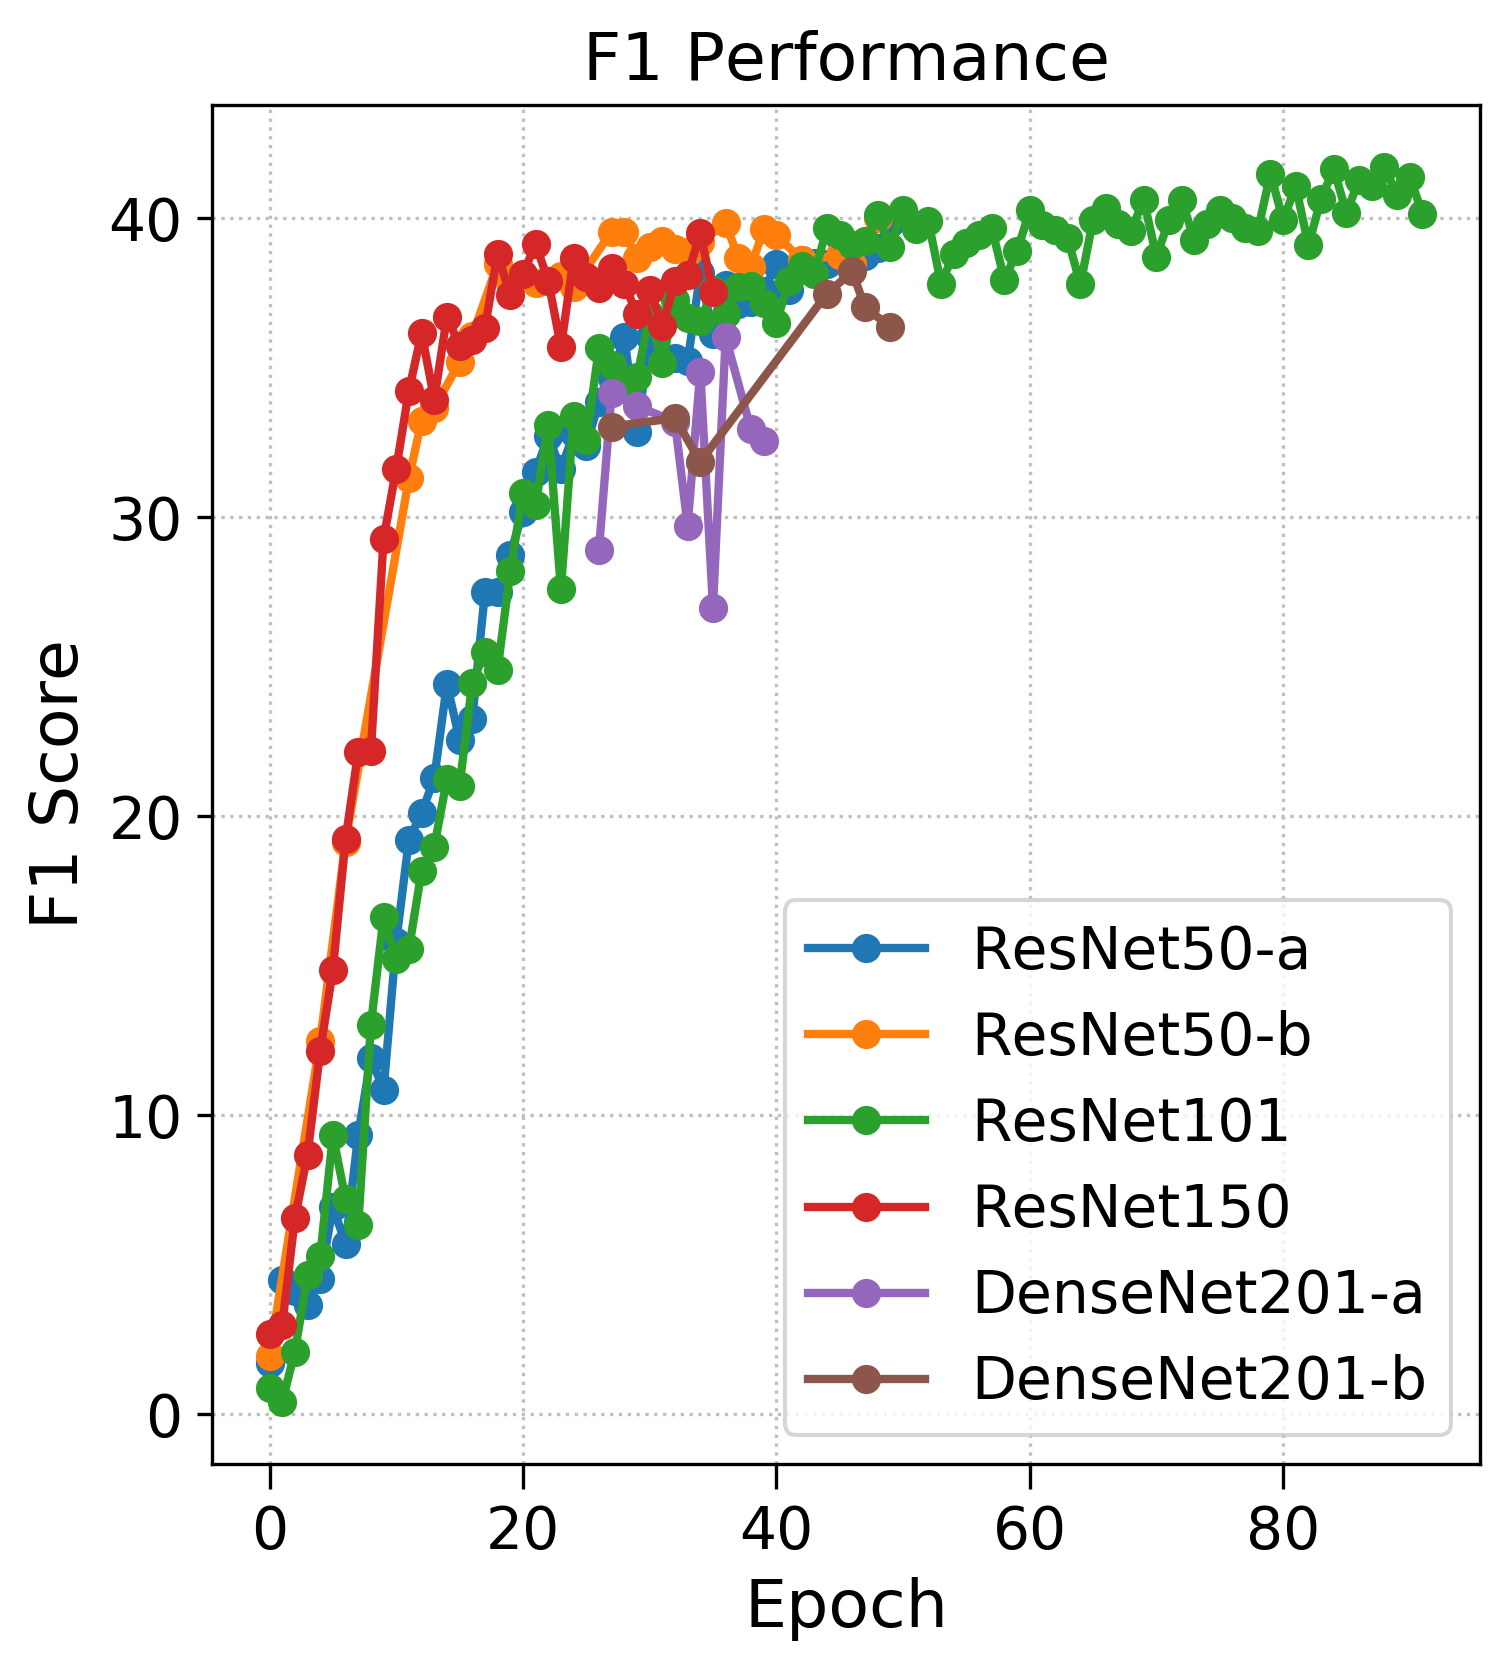
\includegraphics[width=0.9\columnwidth]{images/stemdl/image5b.png}
    \caption{}
    \label{fig:stemdl-f1}
    \end{subfigure}
    \caption{Performance of {\tt stemdl} on the Summit platform.  The classification accuracy and F1-Score against the number of epochs for various hyper-parameter settings are shown in (a) and (b), respectively. See text for more details.}
    \label{fig:stemdl5}
\end{figure}

\begin{figure}[!htb]
    \begin{center}
    \begin{minipage}[b]{0.45\textwidth}
    \centering
    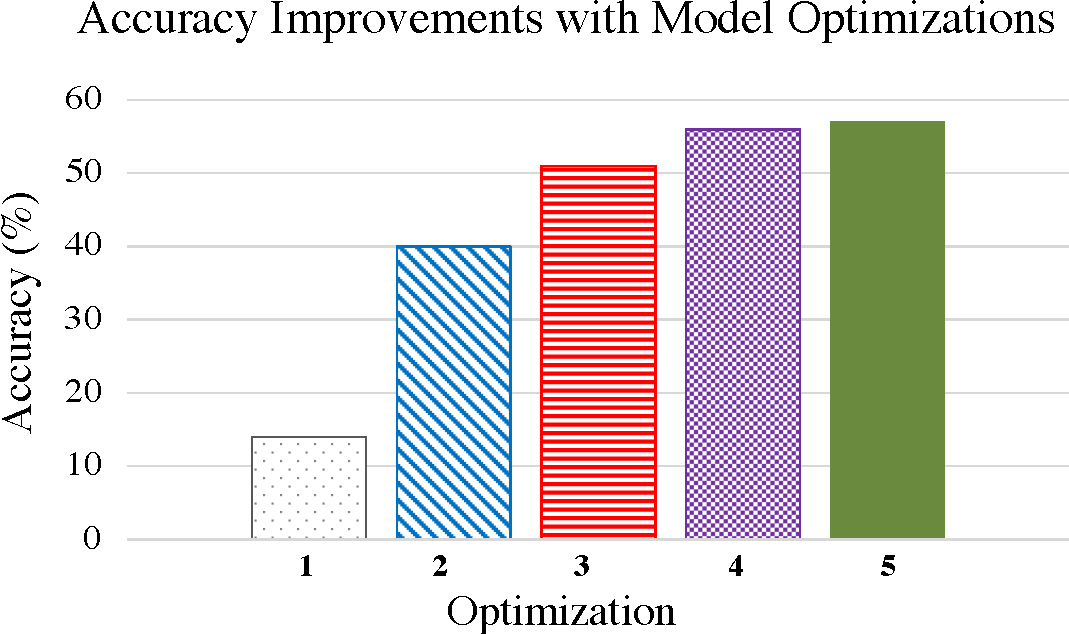
\includegraphics[width=1\columnwidth]{images/stemdl/image6.pdf}
    \caption{Accuracy improvements.}
    \label{fig:stemdl6}
    \end{minipage}
    \hfill
    \begin{minipage}[b]{0.45\textwidth}
    \centering
    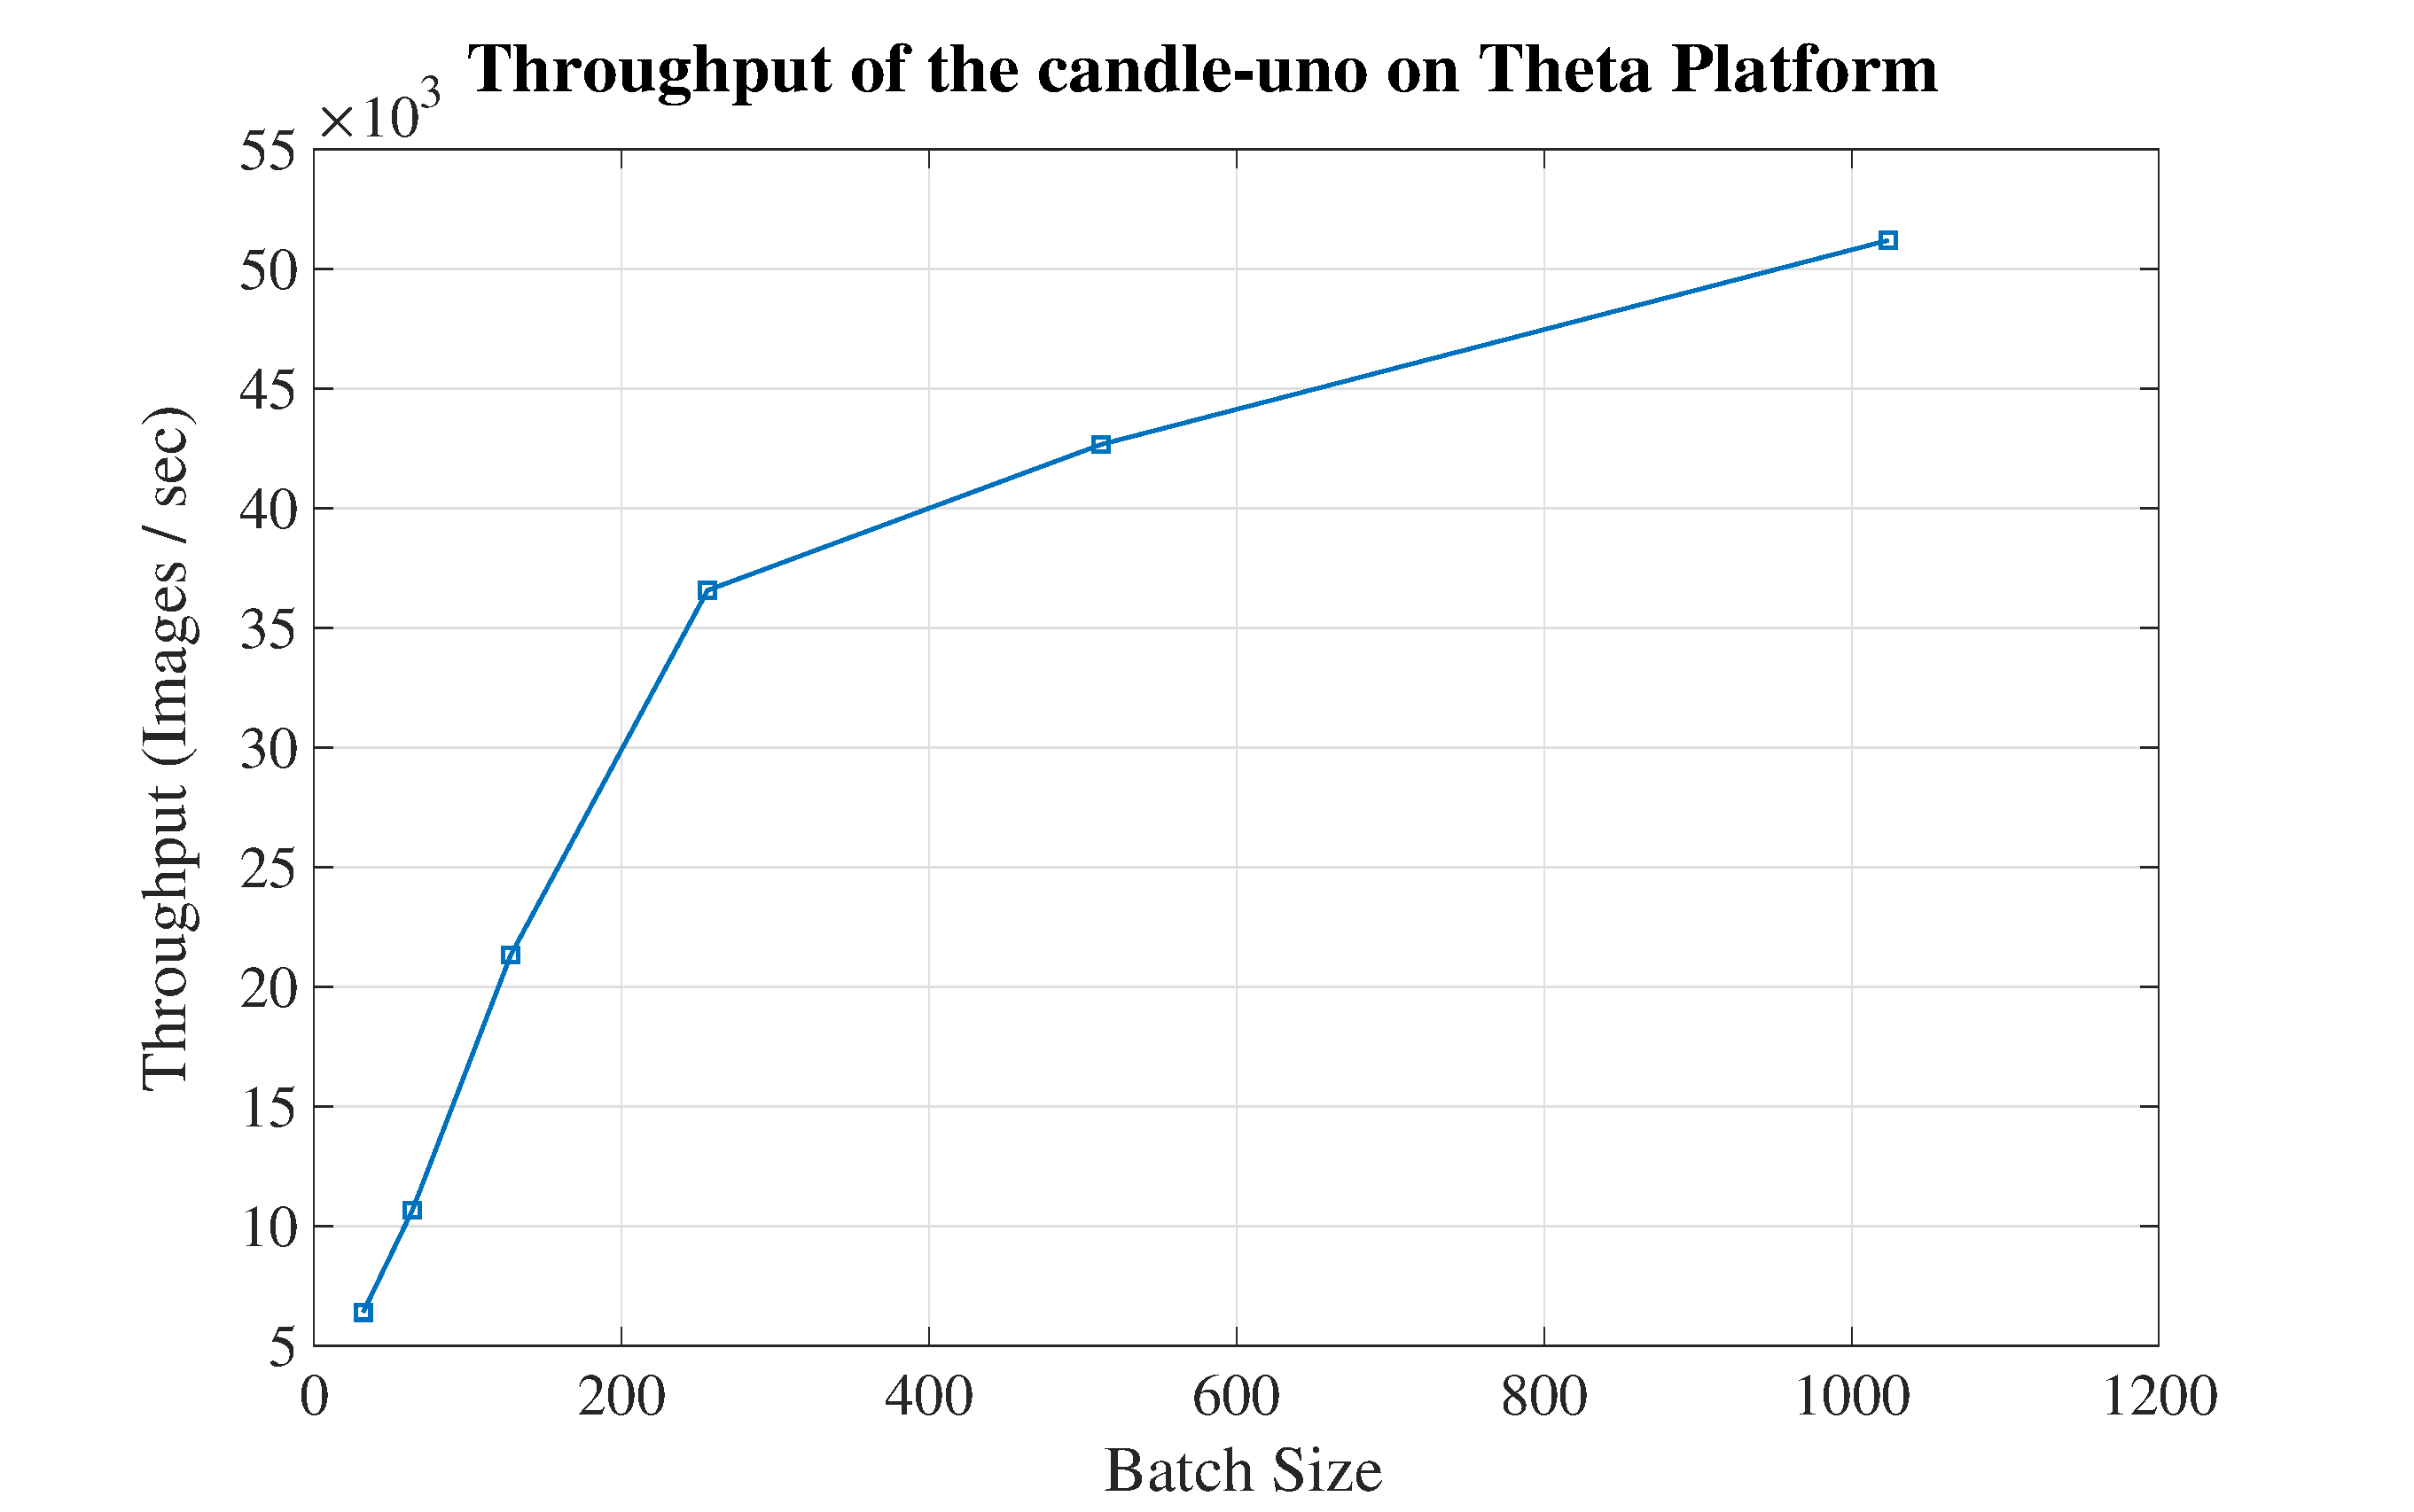
\includegraphics[width=1.0\columnwidth]{images/uno/image7.pdf}
    \caption{Throughput of {\tt candle-uno}.}
    \label{fig:uno-7}
    \end{minipage}
    \end{center}
\end{figure}



%%% Candle-Uno

\subsection{Results for the {\tt candle-uno} Benchmark}

We used the reference implementation on the ThetaGPU platform. As stated before, our metric is throughput (i.e., number of samples processed per second) for varying batch sizes on a single GPU. We present the results in Figure ~\ref{fig:uno-7}. The results show that the the overall throughput increases with the batch size, showing a trend of saturation, and highlights that more investigation is needed to qualify future implementations, especially across different platforms. 


%%% Tevelop

\subsection{Results for the {\tt tevelop} Benchmark}

The {\tt tevelop} benchmark is evaluated by using it to predict earthquakes over the Southern Californian region.  The earthquake data is often binned to generate the spatial time series, and for this evaluation, we  consider the bin size of two-weeks. With this, we used our reference model  with three baseline implementations, namely, LSTM, TFT and Transformer-based models. We first present the performance results of the LSTM-based model focused on science metric in Figure~\ref{fig:eq-2weeks}. The results show that ML can, indeed, offer significant benefits. Additional examples ranging from a week to a year are presented in \cite{fox2022-jm}.

\begin{figure}[!htb]
    \begin{subfigure}{0.49\textwidth}
    \centering
    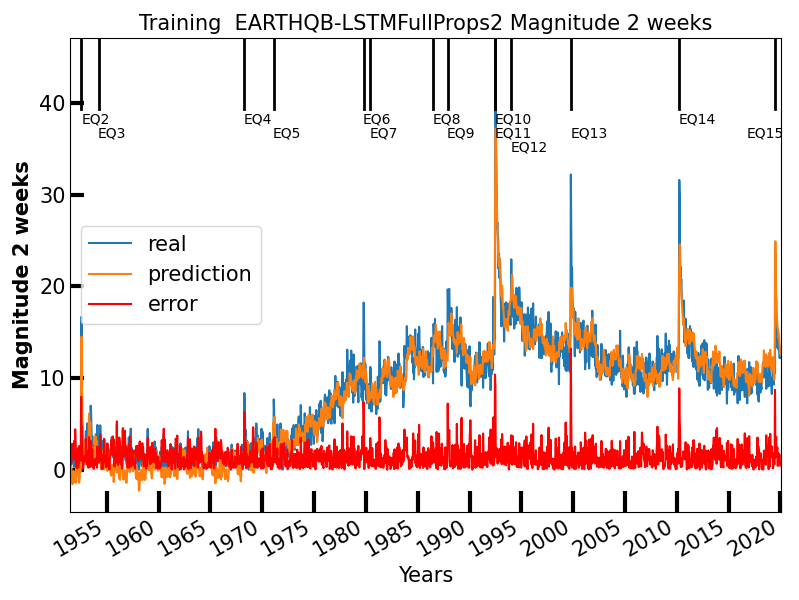
\includegraphics[width=0.8\textwidth]{images/earthquake/image10a.png}
    \caption{}
    \label{fig:tevelop-training}
    \end{subfigure}
    \hfill
    \begin{subfigure}{0.49\textwidth}
    \centering
    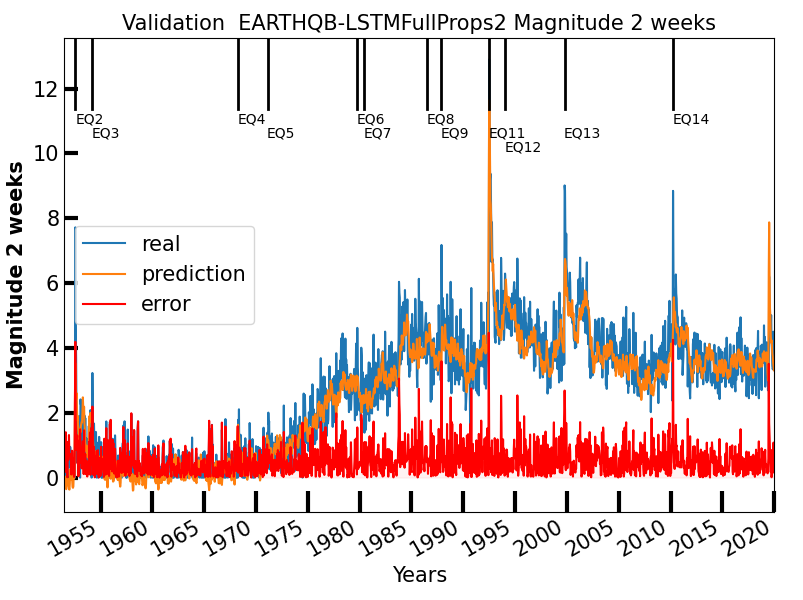
\includegraphics[width=0.8\textwidth]{images/earthquake/image10b.png}
    \caption{}
    \label{fig:tevelop-validation}
    \end{subfigure}
    \caption{Performance of the {\tt tevelop} in predicting earthquakes, for two-week window periods.  The training performance  and the validation accuracy are shown in (a) and (b), respectively covering real and predicted values and the error.}
    \label{fig:eq-2weeks}
\end{figure}


\begin{small}
    \begin{table}
        \caption{Comparison of different models for earthquake prediction.}
        \label{tab:eq-results}
        \begin{center}
        \begin{tabular}{p{2cm}|p{1cm}p{1cm}|p{1cm}p{1cm}|p{1cm}p{1cm}}
        \hline
        \textbf{ }      &  \multicolumn{2}{|c|}{\bf LSTM} & \multicolumn{2}{|c|}{\bf TFT} & \multicolumn{2}{|c}{\bf Transformer}\\
        \textbf{Period} & {\bf Train} & {\bf Test} & {\bf Train} & {\bf Test} & {\bf Train} & {\bf Test}
        \\
        \hline
        \textbf{2 weeks}  & 0.902 & 0.869	& 	0.931	& 	0.885	&	0.893	&	0.856\\
        \textbf{4 weeks}  & 0.896 & 0.883	& 	-		& 	-		&	0.866	&	0.883\\
        \textbf{2 months} & 0.887 & 0.881	& 	-		& 	-		&	0.865	&	0.881\\
        \textbf{3 months} & 0.925 & 0.893	& 	0.976	& 	0.922	&	0.919	&	0.881\\
        \textbf{6 months} & 0.950 & 0.900	& 	0.972	& 	0.882	&	0.954	&	0.896\\
        \textbf{1 year}   & 0.923 & 0.865	& 	0.976	& 	0.853	&	0.955	&	0.876\\
        \textbf{2 years}  & 0.928 & 0.830	& 	-		& 	-		&	0.855	&	0.830\\
        \textbf{4 years}  & 0.937 & 0.770	& 	-		& 	-		&	0.817	&	0.770\\
        \hline
        \end{tabular}
        \end{center}
    \end{table}
    \end{small}

    \begin{figure}[!htb]
        \begin{subfigure}{0.49\textwidth}
        \centering
        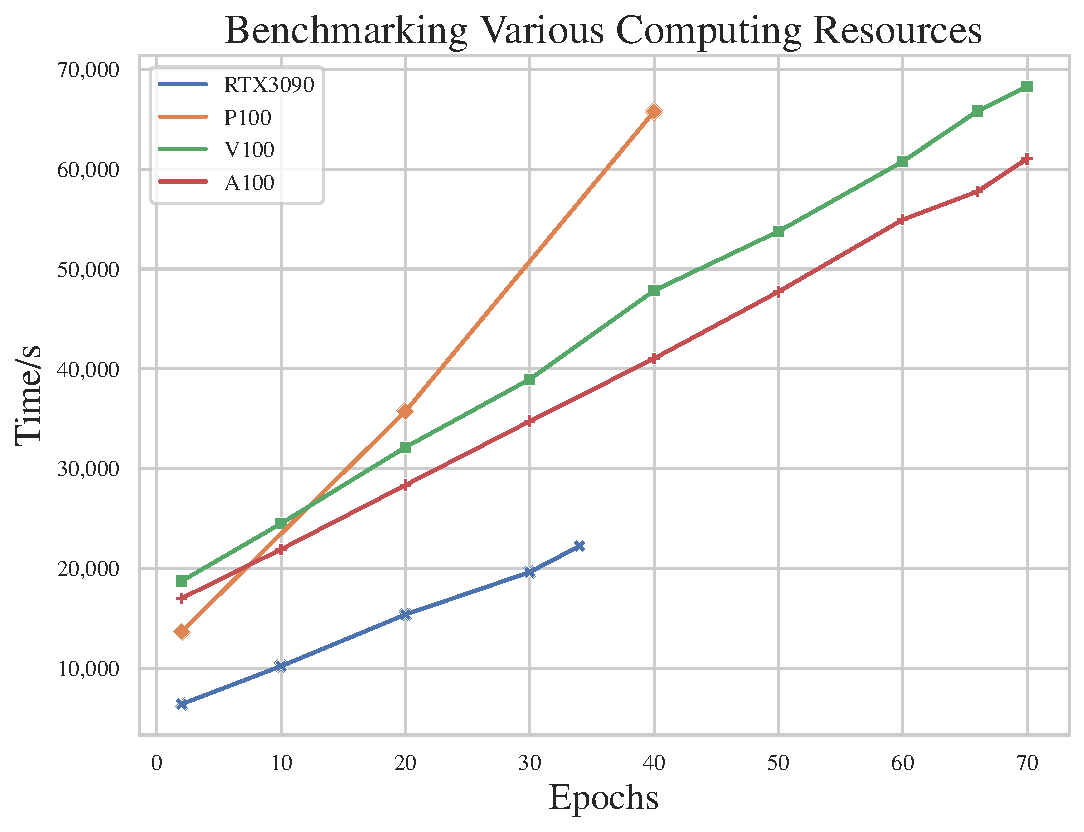
\includegraphics[width=1.0\textwidth]{images/earthquake/eq-compare.pdf}
        \caption{}
        \label{fig:tevelop-runtimes}
        \end{subfigure}
        \hfill
        \begin{subfigure}{0.49\textwidth}
        \centering
        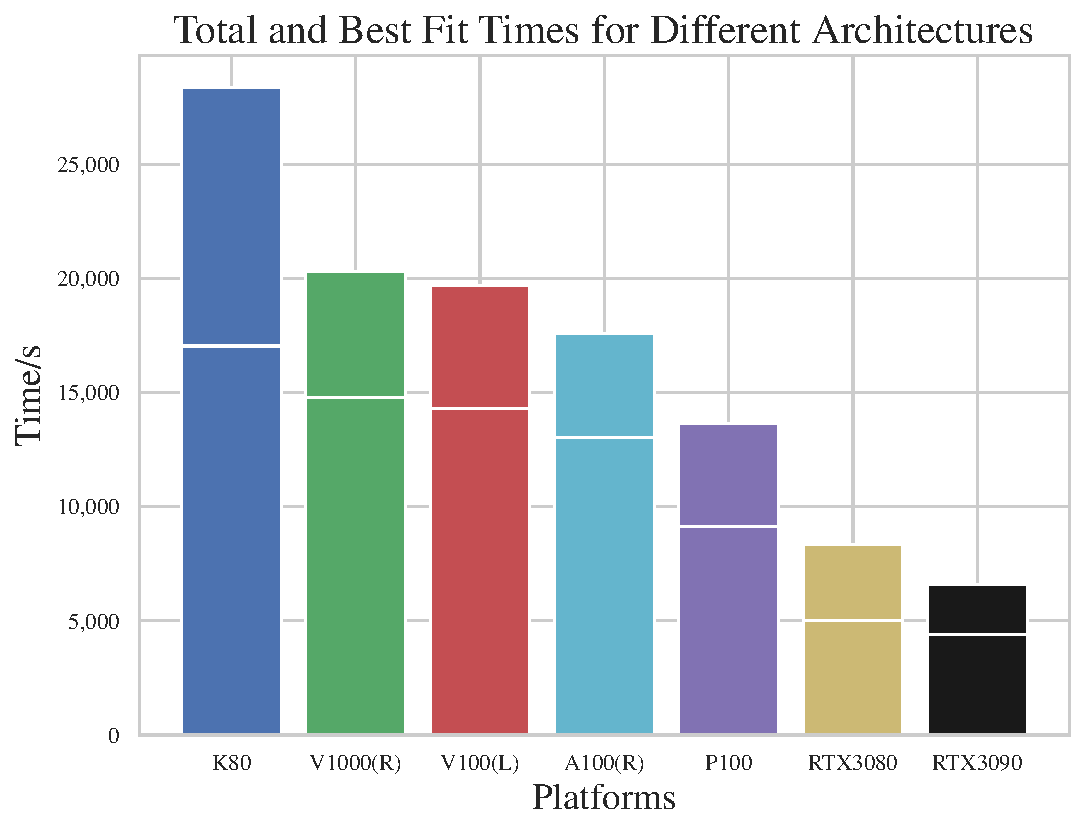
\includegraphics[width=1.0\textwidth]{images/earthquake/storage-performance.pdf}
        \caption{}
        \label{fig:tevelop-disk}
        \end{subfigure}
        \caption{Evaluation of the {\tt tevelop} benchmark across a range of architectures and storage systems.  Figure (a) shows the training performance while (b) shows the impact of different storage systems (such as, local HDD, local NVMe, NFS). }
        \label{fig:tevelop-architectures}
    \end{figure}
    

\noindent To compare and contrast the performance of different baseline models, we use a subset of the full dataset (which has 2,400 pixels) consisting of 500 most active pixels, divided at the ratio of 4:1 for  training and and validation. We then compare these models, across a number of time periods, ranging from two-weeks to four years, and compare their normalized NSE (NNSE) values, with the interpretation of increasing NNSE values imply better predictions. We show the resulting performance in Table~\ref{tab:eq-results}. A more detailed set of examples, and illustrations can be found in~\cite{fox2022-jm}. Finally, we compare the performance of this benchmark on different architectures, and show the results in Figure~\ref{fig:tevelop-architectures}. 










    